\documentclass[english, 11 pt, class=article, crop=false]{standalone}
\usepackage[T1]{fontenc}
%\renewcommand*\familydefault{\sfdefault} % For dyslexia-friendly text
\usepackage{lmodern} % load a font with all the characters
\usepackage{geometry}
\geometry{verbose,paperwidth=16.1 cm, paperheight=24 cm, inner=2.3cm, outer=1.8 cm, bmargin=2cm, tmargin=1.8cm}
\setlength{\parindent}{0bp}
\usepackage{import}
\usepackage[subpreambles=false]{standalone}
\usepackage{amsmath}
\usepackage{amssymb}
\usepackage{esint}
\usepackage{babel}
\usepackage{tabu}
\makeatother
\makeatletter

\usepackage{titlesec}
\usepackage{ragged2e}
\RaggedRight
\raggedbottom
\frenchspacing

% Norwegian names of figures, chapters, parts and content
\addto\captionsenglish{\renewcommand{\figurename}{Figur}}
\makeatletter
\addto\captionsenglish{\renewcommand{\chaptername}{Kapittel}}
\addto\captionsenglish{\renewcommand{\partname}{Del}}


\usepackage{graphicx}
\usepackage{float}
\usepackage{subfig}
\usepackage{placeins}
\usepackage{cancel}
\usepackage{framed}
\usepackage{wrapfig}
\usepackage[subfigure]{tocloft}
\usepackage[font=footnotesize,labelfont=sl]{caption} % Figure caption
\usepackage{bm}
\usepackage[dvipsnames, table]{xcolor}
\definecolor{shadecolor}{rgb}{0.105469, 0.613281, 1}
\colorlet{shadecolor}{Emerald!15} 
\usepackage{icomma}
\makeatother
\usepackage[many]{tcolorbox}
\usepackage{multicol}
\usepackage{stackengine}

\usepackage{esvect} %For vectors with capital letters

% For tabular
\usepackage{array}
\usepackage{multirow}
\usepackage{longtable} %breakable table

% Ligningsreferanser
\usepackage{mathtools}
\mathtoolsset{showonlyrefs}

% index
\usepackage{imakeidx}
\makeindex[title=Indeks]

%Footnote:
\usepackage[bottom, hang, flushmargin]{footmisc}
\usepackage{perpage} 
\MakePerPage{footnote}
\addtolength{\footnotesep}{2mm}
\renewcommand{\thefootnote}{\arabic{footnote}}
\renewcommand\footnoterule{\rule{\linewidth}{0.4pt}}
\renewcommand{\thempfootnote}{\arabic{mpfootnote}}

%colors
\definecolor{c1}{cmyk}{0,0.5,1,0}
\definecolor{c2}{cmyk}{1,0.25,1,0}
\definecolor{n3}{cmyk}{1,0.,1,0}
\definecolor{neg}{cmyk}{1,0.,0.,0}

% Lister med bokstavar
\usepackage[inline]{enumitem}

\newcounter{rg}
\numberwithin{rg}{chapter}
\newcommand{\reg}[2][]{\begin{tcolorbox}[boxrule=0.3 mm,arc=0mm,colback=blue!3] {\refstepcounter{rg}\phantomsection \large \textbf{\therg \;#1} \vspace{5 pt}}\newline #2  \end{tcolorbox}\vspace{-5pt}}

\newcommand\alg[1]{\begin{align} #1 \end{align}}

\newcommand\eks[2][]{\begin{tcolorbox}[boxrule=0.3 mm,arc=0mm,enhanced jigsaw,breakable,colback=green!3] {\large \textbf{Eksempel #1} \vspace{5 pt}\\} #2 \end{tcolorbox}\vspace{-5pt} }

\newcommand{\st}[1]{\begin{tcolorbox}[boxrule=0.0 mm,arc=0mm,enhanced jigsaw,breakable,colback=yellow!12]{ #1} \end{tcolorbox}}

\newcommand{\spr}[1]{\begin{tcolorbox}[boxrule=0.3 mm,arc=0mm,enhanced jigsaw,breakable,colback=yellow!7] {\large \textbf{Språkboksen} \vspace{5 pt}\\} #1 \end{tcolorbox}\vspace{-5pt} }

\newcommand{\sym}[1]{\colorbox{blue!15}{#1}}

\newcommand{\info}[2]{\begin{tcolorbox}[boxrule=0.3 mm,arc=0mm,enhanced jigsaw,breakable,colback=cyan!6] {\large \textbf{#1} \vspace{5 pt}\\} #2 \end{tcolorbox}\vspace{-5pt} }

\newcommand\algv[1]{\vspace{-11 pt}\begin{align*} #1 \end{align*}}

\newcommand{\regv}{\vspace{5pt}}
\newcommand{\mer}{\textsl{Merk}: }
\newcommand{\mers}[1]{{\footnotesize \mer #1}}
\newcommand\vsk{\vspace{11pt}}
\newcommand\vs{\vspace{-11pt}}
\newcommand\vsb{\vspace{-16pt}}
\newcommand\sv{\vsk \textbf{Svar} \vspace{4 pt}\\}
\newcommand\br{\\[5 pt]}
\newcommand{\figp}[1]{../fig/#1}
\newcommand\algvv[1]{\vs\vs\begin{align*} #1 \end{align*}}
\newcommand{\y}[1]{$ {#1} $}
\newcommand{\os}{\\[5 pt]}
\newcommand{\prbxl}[2]{
\parbox[l][][l]{#1\linewidth}{#2
	}}
\newcommand{\prbxr}[2]{\parbox[r][][l]{#1\linewidth}{
		\setlength{\abovedisplayskip}{5pt}
		\setlength{\belowdisplayskip}{5pt}	
		\setlength{\abovedisplayshortskip}{0pt}
		\setlength{\belowdisplayshortskip}{0pt} 
		\begin{shaded}
			\footnotesize	#2 \end{shaded}}}

\renewcommand{\cfttoctitlefont}{\Large\bfseries}
\setlength{\cftaftertoctitleskip}{0 pt}
\setlength{\cftbeforetoctitleskip}{0 pt}

\newcommand{\bs}{\\[3pt]}
\newcommand{\vn}{\\[6pt]}
\newcommand{\fig}[1]{\begin{figure}
		\centering
		\includegraphics[]{\figp{#1}}
\end{figure}}

\newcommand{\figc}[2]{\begin{figure}
		\centering
		\includegraphics[]{\figp{#1}}
		\caption{#2}
\end{figure}}

\newcommand{\sectionbreak}{\clearpage} % New page on each section

\newcommand{\nn}[1]{
\begin{equation}
	#1
\end{equation}
}

% Equation comments
\newcommand{\cm}[1]{\llap{\color{blue} #1}}

\newcommand\fork[2]{\begin{tcolorbox}[boxrule=0.3 mm,arc=0mm,enhanced jigsaw,breakable,colback=yellow!7] {\large \textbf{#1 (forklaring)} \vspace{5 pt}\\} #2 \end{tcolorbox}\vspace{-5pt} }
 
%colors
\newcommand{\colr}[1]{{\color{red} #1}}
\newcommand{\colb}[1]{{\color{blue} #1}}
\newcommand{\colo}[1]{{\color{orange} #1}}
\newcommand{\colc}[1]{{\color{cyan} #1}}
\definecolor{projectgreen}{cmyk}{100,0,100,0}
\newcommand{\colg}[1]{{\color{projectgreen} #1}}

% Methods
\newcommand{\metode}[2]{
	\textsl{#1} \\[-8pt]
	\rule{#2}{0.75pt}
}

%Opg
\newcommand{\abc}[1]{
	\begin{enumerate}[label=\alph*),leftmargin=18pt]
		#1
	\end{enumerate}
}
\newcommand{\abcs}[2]{
	\begin{enumerate}[label=\alph*),start=#1,leftmargin=18pt]
		#2
	\end{enumerate}
}
\newcommand{\abcn}[1]{
	\begin{enumerate}[label=\arabic*),leftmargin=18pt]
		#1
	\end{enumerate}
}
\newcommand{\abch}[1]{
	\hspace{-2pt}	\begin{enumerate*}[label=\alph*), itemjoin=\hspace{1cm}]
		#1
	\end{enumerate*}
}
\newcommand{\abchs}[2]{
	\hspace{-2pt}	\begin{enumerate*}[label=\alph*), itemjoin=\hspace{1cm}, start=#1]
		#2
	\end{enumerate*}
}

% Oppgaver
\newcommand{\opgt}{\phantomsection \addcontentsline{toc}{section}{Oppgaver} \section*{Oppgaver for kapittel \thechapter}\vs \setcounter{section}{1}}
\newcounter{opg}
\numberwithin{opg}{section}
\newcommand{\op}[1]{\vspace{15pt} \refstepcounter{opg}\large \textbf{\color{blue}\theopg} \vspace{2 pt} \label{#1} \\}
\newcommand{\ekspop}[1]{\vsk\textbf{Gruble \thechapter.#1}\vspace{2 pt} \\}
\newcommand{\nes}{\stepcounter{section}
	\setcounter{opg}{0}}
\newcommand{\opr}[1]{\vspace{3pt}\textbf{\ref{#1}}}
\newcommand{\oeks}[1]{\begin{tcolorbox}[boxrule=0.3 mm,arc=0mm,colback=white]
		\textit{Eksempel: } #1	  
\end{tcolorbox}}
\newcommand\opgeks[2][]{\begin{tcolorbox}[boxrule=0.1 mm,arc=0mm,enhanced jigsaw,breakable,colback=white] {\footnotesize \textbf{Eksempel #1} \\} \footnotesize #2 \end{tcolorbox}\vspace{-5pt} }
\newcommand{\rknut}{
Rekn ut.
}

%License
\newcommand{\lic}{\textit{Matematikken sine byggesteinar by Sindre Sogge Heggen is licensed under CC BY-NC-SA 4.0. To view a copy of this license, visit\\ 
		\net{http://creativecommons.org/licenses/by-nc-sa/4.0/}{http://creativecommons.org/licenses/by-nc-sa/4.0/}}}

%referances
\newcommand{\net}[2]{{\color{blue}\href{#1}{#2}}}
\newcommand{\hrs}[2]{\hyperref[#1]{\color{blue}\textsl{#2 \ref*{#1}}}}
\newcommand{\rref}[1]{\hrs{#1}{regel}}
\newcommand{\refkap}[1]{\hrs{#1}{kapittel}}
\newcommand{\refsec}[1]{\hrs{#1}{seksjon}}

\newcommand{\mb}{\net{https://sindrsh.github.io/FirstPrinciplesOfMath/}{MB}}


%line to seperate examples
\newcommand{\linje}{\rule{\linewidth}{1pt} }

\usepackage{datetime2}
%%\usepackage{sansmathfonts} for dyslexia-friendly math
\usepackage[]{hyperref}


\newcounter{inl}
\numberwithin{inl}{chapter}
\newcommand{\inl}[1]{\vspace{15pt} \refstepcounter{inl} \textbf{Oppgave \theinl}\label{#1} \vspace{2 pt}\\}
\renewcommand\theinl{\arabic{inl}}

\newcommand{\inr}[1]{\vspace{3pt}\textbf{\ref{#1}}}
\begin{document}
{\textbf{\Large Øving for prøve i kapittel 5-7 (fredag 3. nov.)}}\\ \vspace{5 pt}

\inl{in1}
Gjør om:\os
\begin{tabular}{@{}l l l l}
	\textbf{a)} 14\,m til lengde målt i km.\\
	\textbf{b)} 25000\,m til lengde målt i mil.\\
	\textbf{c)} 23,5\,mm til lengde målt i dm.
\end{tabular}

\inl{in2}

Gjør om:\os
\begin{tabular}{@{}l l l l}
	\textbf{a)} 145\,m$ ^2 $ til areal målt i km$ ^2 $.\\
	\textbf{b)} 28000\,m$ ^2 $ til areal målt i dm$ ^2 $.\\
	\textbf{c)} 223,5\,mm$ ^2 $ til areal målt i dm$ ^2 $.
\end{tabular}

\inl{in3}

I en klasse er det 21 personer som kjører til skolen og 10 som tar båt. Hva er forholdet mellom antall personer som kjører og tar båt?

\inl{in4}
Du lager et lotteri og ønsker at forholdet mellom antall vinnerlodd og taperlodd skal være $ {2:7} $. Hvis du lager 12 vinnerlodd, hvor mange taperlodd må du da lage?

\inl{in5}
I en twistpose er det 15 sjokolader igjen, alle av de to beste sortene, som er \textsl{Marsipan} og \textsl{Cocos}. Forholdet mellom \textsl{Marsipan} og \textsl{Cocos} i posen er $ {1:4} $.\os
\textbf{a)} Hvor mange \textsl{Marsipan} og hvor mange \textsl{Cocos} ligger i posen?\os
\textbf{b)} Etter en stund har forholdet endret seg til $ {1:3} $. Hva kan ha skjedd?

\inl{in6}
Trekant $ \triangle ABC $ inneholder vinklene  $ 35^\circ $ og $ 60^\circ $, mens $ \triangle DEF $ inneholder vinklene  $ 85^\circ $ og $ 40^\circ $.\os
\textbf{a)} Finn den resterende vinkelen i begge trekantene.\os
\textbf{b)} Er trekantene formlike?
\newpage
\inl{in7}
\fig{tri4}
\textbf{a)} Forklar (NØYE!) hvorfor trekantene $ \triangle ABC $ og $ \triangle ADC $ er formlike. Lag en tegning som viser hvor på figuren man kan finne $ \angle A, \angle B $ og $ \angle C $.\os
\textbf{b)} Hvilke sider i trekantene er samsvarende?\os
\textbf{c)} \y{AB=10}, \y{BC=6} og \y{AC=8}. Forklar hvorfor høyden til $ \triangle ABC $ er 4,8.\os
\textbf{d)} Hva er arealet til $ \triangle ABC $?\os
\textbf{e)} Hva er arealet til $ \triangle ADC $?

\inl{in8}
\textbf{a)} Skriv om arealformelen for en trekant til en formel for grunnlinjen $ g $. Hva er $ g $ hvis $ {h=4} $ og \y{A=12}?\os
\textbf{b)} Skriv om arealformelen for et trapes til en formel for $ a $. Hva er $ a $ hvis $ {h=3, b=3} $ og $ A= 15$?\os
\textbf{c)} Skriv om arealformelen for et trapes til en formel for $ h $. Hva er $ h $ hvis $ {a=3, b=7} $ og $ {A=25} $?\os
\textbf{d)} Skriv om omkretsformelen for en sirkel til en formel for radiusen $ r $. Hva er $ r $ hvis $ {O=12\pi} $?
\newpage
\inl{in9}
Linjalen på bildet er en klassisk linjal med cm-mål.
\begin{figure}
	\centering
	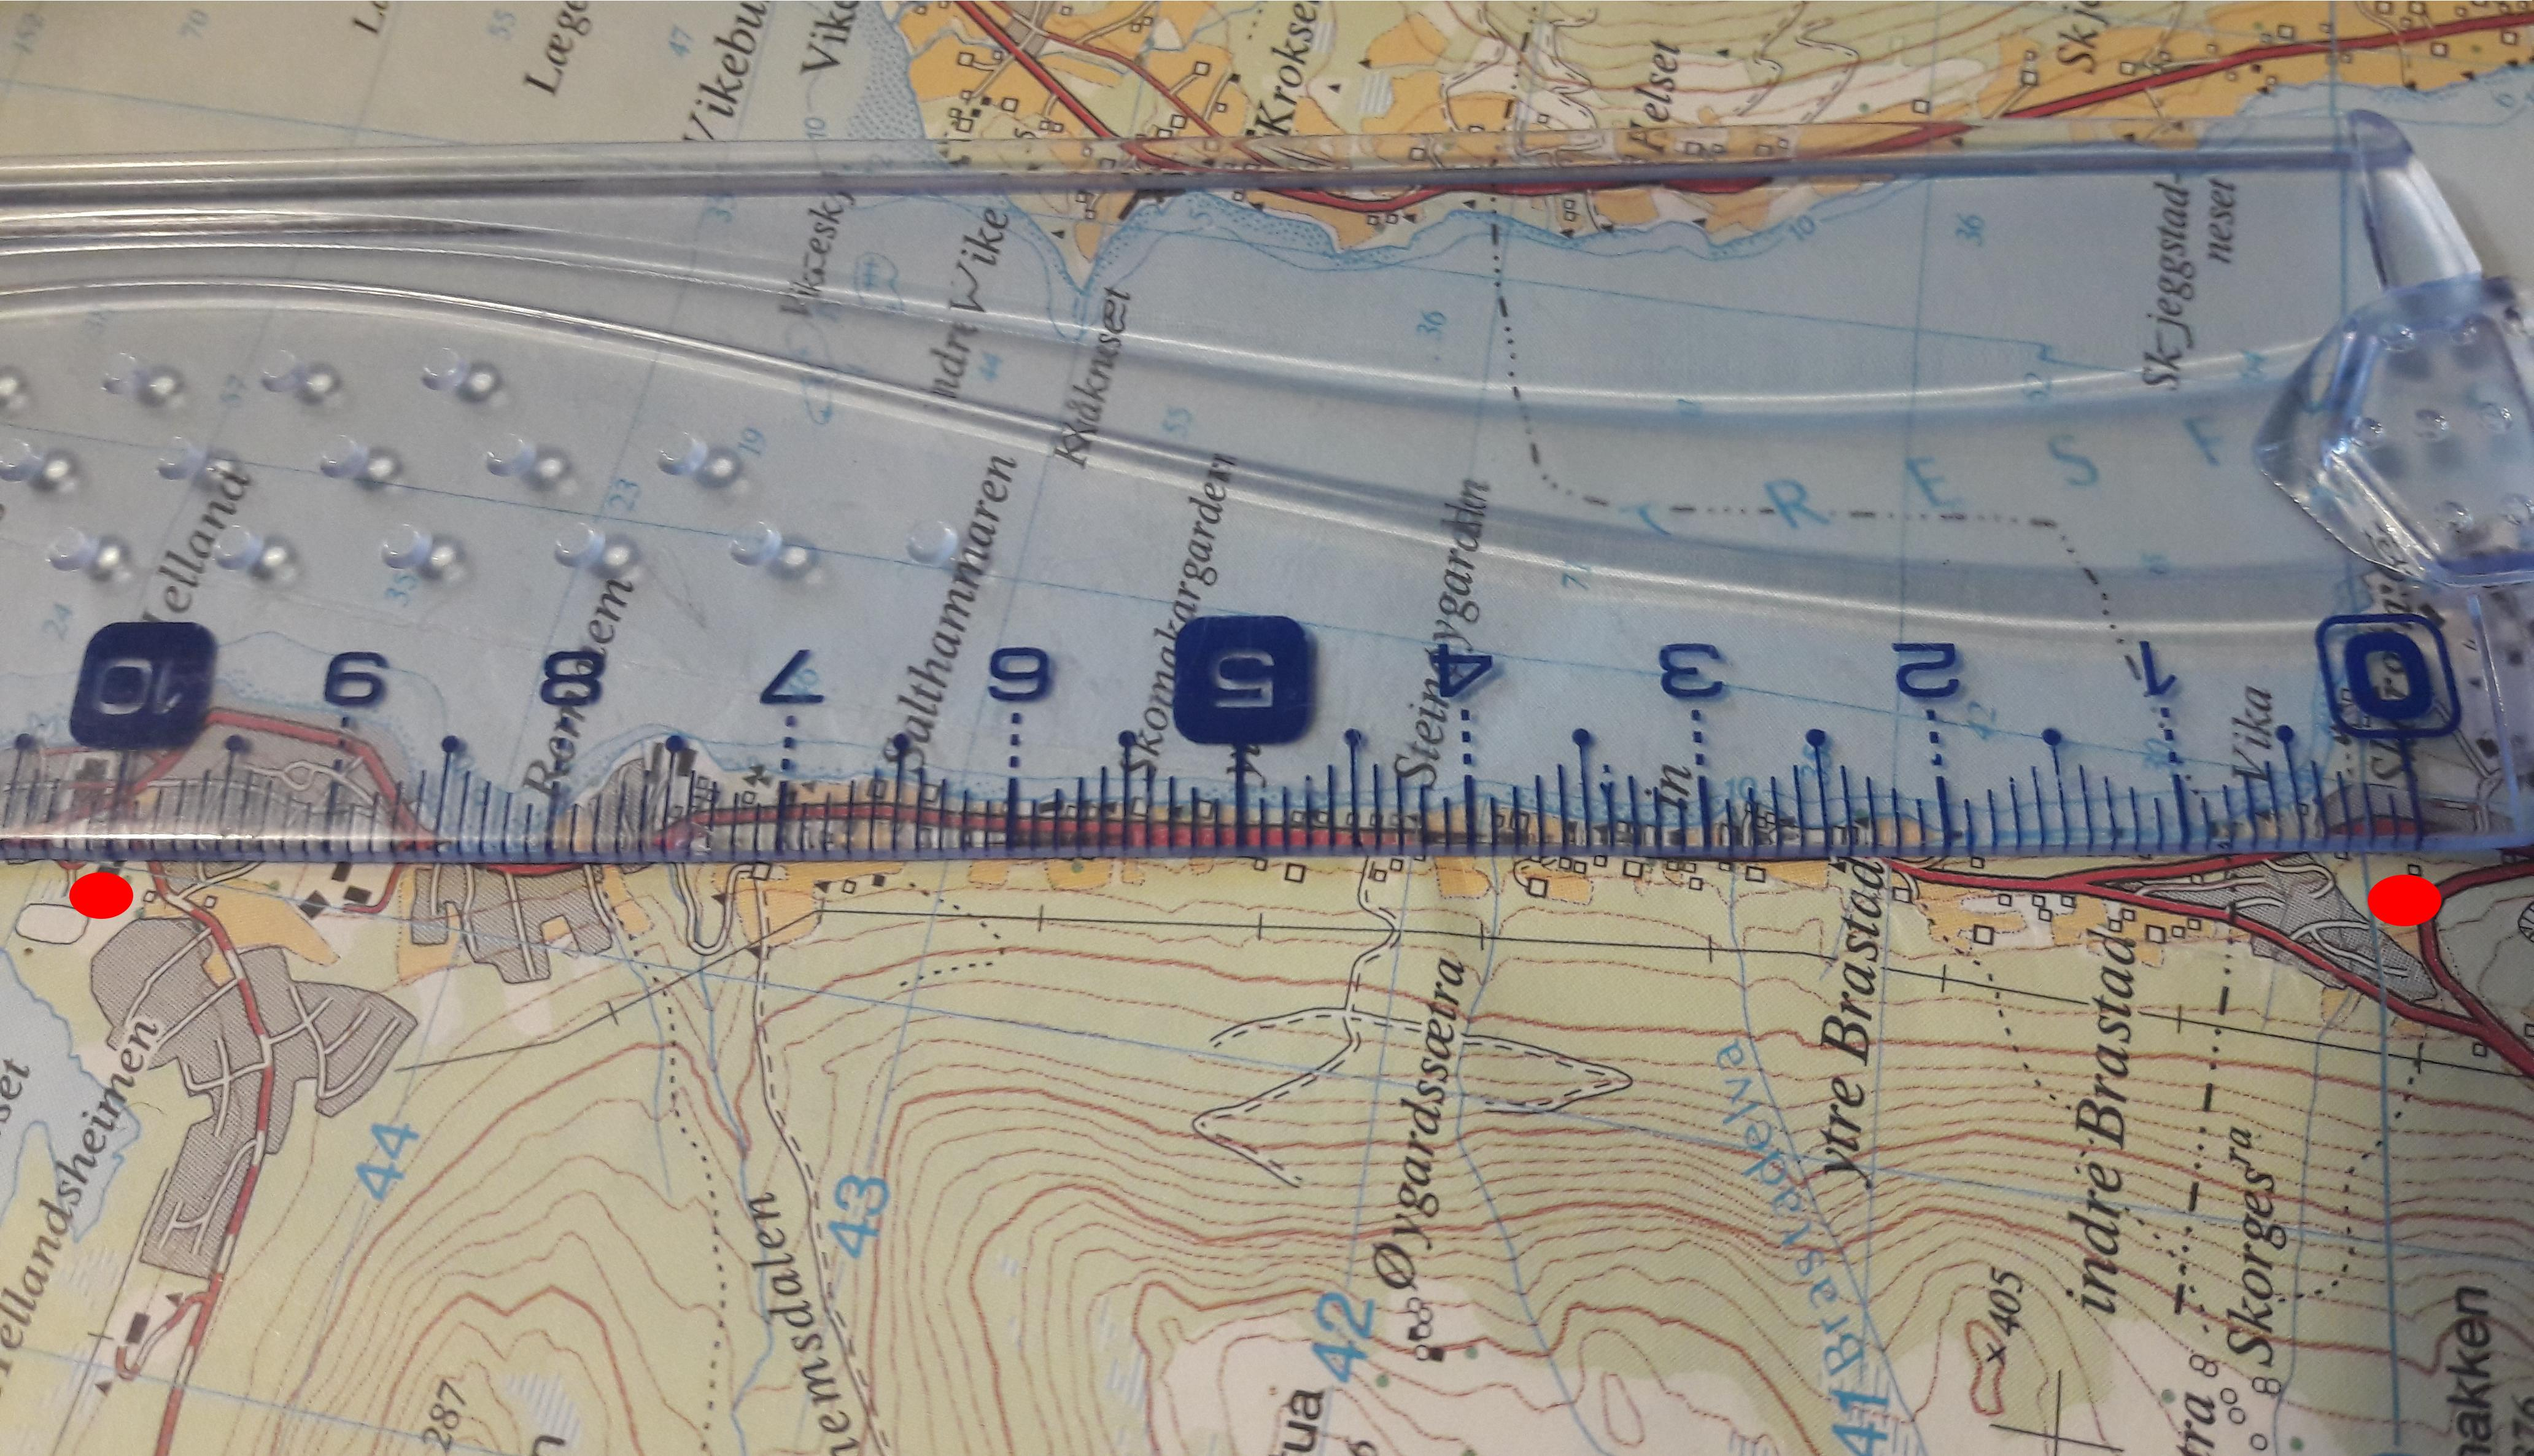
\includegraphics[scale=0.08]{kart}
\end{figure}
På kartet over er huset til Sindre markert med den røde prikken til høyre, og Helland skule (ungdomsskolen i Vestnes) markert med den røde prikken til venstre. Kartet er i målestokken $ {1:50\,000} $.\os
\textbf{a)} Hvor langt er det mellom huset til Sindre og Helland skule?\os

\textbf{b)} Etter at dette kartet ble lagd, har en bro blitt bygget over Tresfjorden (fjorden på kartet). Broen er ca 2\,km lang i virkeligheten. Hvor lang blir denne broen på kartet?

\inl{in10}
I denne oppgaven bruker vi at $ \pi\approx 3 $.\os

En idrettsbane har mål som vist i figuren under:
\fig{tri25}
\textbf{a)} Finn omkretsen til idrettsbanen. Vurder om svaret du finner virker rimelig.\os
\textbf{b)} Finn arealet til idrettsbanen.
\newpage
\inl{in11}
\textbf{a)} Skriv om arealformelen for en sirkel til en formel for radiusen $ r $.\os
\textbf{d)} Hvis en sirkel har arealet $ 36\pi $, hva er da radiusen til sirkelen?

\inl{in12}
I en bøtte med 21\,L maling er det blandet grønn og rød maling i forholdet $ {2:5} $.\os
\textbf{a)} Hvor mye grønn maling er det i bøtten?\os

\textbf{b)} Hvor mye rød maling er det i bøtten?\os

\textbf{c)} Hva kan du gjøre for å endre forholdet til $ 2:9 $?\os
\textbf{d)} Hva kan du gjøre for å endre forholdet til $ 1:2 $?

\newpage
\section*{Løsningsforslag}
\inr{in1} \os

\begin{tabular}{@{}l l l l}
	\textbf{a)} $ 14\enh{m}=0,014\enh{km} $\\
	\textbf{b)} $ 25000\enh{m}=2,5\enh{mil} $\\
	\textbf{c)} $ 23,5\enh{mm}=0,235\enh{dm} $
\end{tabular}\vsk

\inr{in2}\os
\begin{tabular}{@{}l l l l}
	\textbf{a)} $ 145\enh{m}^2=0,000145\enh{km}^2 $.\\
	\textbf{b)} $ 28\,000\enh{m}^2=2\,800\,000\enh{dm}^2 $\\
	\textbf{c)} $ 223,5\enh{mm}^2=0,02235\enh{dm}^2 $.
\end{tabular}\vsk

\inr{in3}
Forholdet er:
\alg{
\frac{\text{antall som kjører til skolen}}{\text{antall som tar båt}}&=	
\frac{21}{10}\\&=2,1
}

\inr{in4}
Vi vet at:
\alg{
\frac{\text{vinnerlodd}}{\text{taperlodd}}&= \frac{2}{7}
}
12 vinnerlodd er 6 ganger mer enn 2. Det betyr at vi må ha 6 ganger flere taperlodd for at forholdet skal bli det samme:
\alg{
\frac{2\cdot 6}{7\cdot 6}&= \frac{12}{42}
}
Vi må altså lage 42 taperlodd.\vsk

\inr{in5}\\
\textbf{a)}
Siden forholdet er $ {1:4} $ er det $ {1+4=5} $ deler i alt. Det betyr at det er $ {15\cdot\frac{1}{5}=}3 $ \textsl{Marsipan} og $ {15\cdot\frac{4}{5}=12} $ \textsl{Cocos}.\os
\textbf{b)} 
\begin{itemize}
	\item Det kan ha blitt spist 3 \textsl{Cocos}. For da er forholdet $ {\frac{3}{9}=\frac{1}{3}} $.
	\item Det kan ha blitt spist 2 \textsl{Marsipan} og 9 \textsl{Cocos}. For da er forholdet $ {\frac{1}{3}} $.	
	\item Det kan ha blitt spist én \textsl{Marsipan} og 6 \textsl{Cocos}. For da er forholdet $ {\frac{2}{6}=\frac{1}{3}} $
\end{itemize} \vsk

\inr{in6}\\
\textbf{a)} For $ \triangle ABC $:
\alg{
180^\circ-35^\circ-60^\circ&= 85^\circ
}
For $ \triangle DEF $:
\alg{
	180^\circ-85^\circ-40^\circ&= 55^\circ
}
\textbf{b)} Trekantene har forskjellige vinkelverdier og er derfor ikke formlike.\vsk

\inr{in7}\\
(Noen ganger kan det være lurt å tegne trekantene hver for seg for et tydeligere bilde:)
\begin{figure}
	\centering
	\subfloat{\includegraphics[scale=0.7]{\asym{tri4a}}}\quad
	\subfloat{\includegraphics[scale=0.7]{\asym{tri4b}}}
\end{figure}
\textbf{a)} 
\begin{itemize}
	\item Trekantene deler $ \angle A $
	\item Begge trekantene har en $ 90^\circ $ vinkel.
	\item Trekantene har derfor to samsvarende vinkelverdier, og er da formlike.
\end{itemize}

\textbf{b)}\vs \vs
\begin{figure}
	\centering
	\subfloat{\includegraphics[scale=0.7]{\asym{tri4c}}}\quad
	\subfloat{\includegraphics[scale=0.7]{\asym{tri4d}}}
\end{figure}
\begin{itemize}
	\item $ AB $ og $ AC $ er samsvarende (hører til $ 90^\circ $-graderen).
	\item $ BC $ og $ DC $ er samsvarende (hører til $ \angle A $).	
	\item $ AC $ og $ AD $ er samsvarende (hører til $ \angle B $).		
\end{itemize}
\textbf{c)} Høyden i $ \triangle ABC $ er lengden av $ DC $. Av det vi fant i oppgave b) og \hr{forform} vet vi at:
\alg{
\frac{AC}{AB} &= \frac{DC}{BC} \\
\frac{8}{10}&= \frac{DC}{6} \\
\frac{8\cdot 6}{10}&= \frac{DC\cdot \cancel{6}}{\cancel{6}} \\
\frac{48}{10}&= DC \\
4,8 &= DC
}
Derfor er høyden 4,8.\os

\textbf{c)} $ \triangle ABC $ har grunnlinjen $ {AB=10} $ og høyden $ {DC=4,8} $:
\alg{
A &= \frac{g\cdot h}{2}\br
&= \frac{10\cdot4,8}{2}\br
&= \frac{48}{2}\\
&= 24
}

\textbf{d)} Hvis vi velger oss $ {AD} $ som grunnlinje i $ \triangle DEF $ blir høyden $ {DC=4,8} $. Lengde til $ AD $ kan vi finne på lignende måte som i opg b):
\alg{
\frac{AD}{AC}&= \frac{DC}{BC} \br
\frac{AD}{8}&= \frac{4,8}{6} \br
\frac{AD\cdot \cancel{8}}{\cancel{8}}&= \frac{4,8\cdot8}{6} \br
AD &= \frac{38,4}{6} \\
 &= 6,4
}
Arealet blir derfor: \vs
\alg{
	A &= \frac{6,4\cdot 4,8}{2}\br
	&= \frac{10\cdot4,8}{2}\br
	&= \frac{48}{2}\\
	&= 24
}\vsk

\inr{in8}\\
\textbf{a)} Vi skriver om arealformelen slik at $ h $ står alene på én side: 
\alg{
A &= \frac{g\cdot h}{2} \br
2\cdot A &= \frac{\cancel{2}\cdot g\cdot h}{\cancel{2}} \br
\frac{2A}{h} &= \frac{g\cdot \cancel{h}}{\cancel{h}} \br
\frac{2A}{h} &= g
}
Når vi vet at $ {h=4} $ og \y{A=12} kan vi bruke formelen over tl å finne $ g $:
\alg{
g &= \frac{2\cdot 12}{4} \\
 &= 6
}

\textbf{b)} Vi skriver om arealformelen slik at $ a $ står alene på én side: 
\alg{
	A &= \frac{a+b}{2} \br
	2\cdot A &= \frac{\cancel{2}\cdot g\cdot h}{\cancel{2}} \br
	\frac{2A}{h} &= \frac{g\cdot \cancel{h}}{\cancel{h}} \br
	\frac{2A}{h} &= g
}
Når vi vet at $ {h=4} $ og \y{A=12} kan vi bruke formelen over tl å finne $ g $:
\alg{
	g &= \frac{2\cdot 12}{4} \\
	&= 6
}
\textbf{b)} Vi skriver om arealformelen slik at $ a $ står alene på én side: 
\alg{
	A &= \frac{(a+b)h}{2} \br
	2\cdot A &=\cancel{2}\cdot\frac{(a+b)h}{\cancel{2}} \br
	\frac{2A}{h} &= \frac{(a+b)\cancel{h}}{\cancel{h}}\br
	\frac{2A}{h}-b &= a
}
Når vi vet at $ {h=3, b=3} $ og $ A= 15$ kan vi bruke formelen over til å finne $ a $:
\alg{
 a &= \frac{2\cdot 15}{3}-3 \\
 &= \frac{30}{3}-3 \\
 &= 10-3\\
 &= 7
}\os

\textbf{c)} Vi skriver om arealformelen slik at $ h $ står alene på én side: 
\alg{
	A &= \frac{(a+b)h}{2} \br
	2\cdot A &=\cancel{2}\cdot\frac{(a+b)h}{\cancel{2}} \br
	\frac{2A}{(a+b)} &= \frac{\bcancel{(a+b)}h}{{\bcancel{(a+b)}}}\br
	\frac{2A}{(a+b)} &= h
}
Når vi vet at $ {a=3, b=7} $ og $ A= 25$ kan vi bruke formelen over til å finne $ h $:
\alg{
h &= \frac{2\cdot 25}{(3+7)} \\
&= \frac{50}{10} \\
&= 5
}

\inr{in9} \\
\textbf{a)} På karter er det 10\,cm mellom huset og skolen. Målestokken sier at \textsl{én cm på kartet er 50\,000} i virkeligheten, altså at:
\alg{
	\text{10\,cm i virkeligheten}&= 10\cdot 50\,000\text{\,cm i virkeligheten} \\ 
	&= 500\,000\text{\,cm i virkeligheten} \\
	&= 5\enh{km}
}
Det er altså 5\,km mellom skolen og huset.\os

\textbf{b)} Målestokken forteller at:
\alg{
	\frac{\text{lengde på kart}}{\text{lengde i virkeligheten}}&= \frac{1}{50\,000} \br
	\frac{\text{lengde på kart}}{\text{2\,km}}&= \frac{1}{50\,000} \br
	\text{lengde på kart} &= \frac{200\,000\enh{cm}}{50\,000}\\
	&= 4\enh{cm}
}

\inr{in10}
Idrettsbanen består av to halvsirkler, begge med 40\,m radius, og to lengder, begge 80\,m. Da to halvsirklene kan vi slå sammen til én sirkel, som har omkretsen $O_s= 2\pi r $. Altså er:
\alg{
	O_s&=2\pi\cdot40 \\
	&\approx 2\cdot3\cdot40 \\
	&= 240
}
Omkretsen av hele løpebanen blir derfor:
\[ 240+80+80=400 \]
Det er derfor 400\,m rundt banen, noe som gir mening siden det er en idrettsbane. \vsk

\inr{in12}\\
\textbf{a)} Siden forholdet er $ {2:5} $ er det i alt $ {2+5=7} $ deler. Den grønne malingen utgjør derfor $ \frac{2}{7} $ av 21\,L som er:
\[ \frac{2}{7}\cdot21\,L =6\,L \] 
\textbf{b)} Siden det er 6\,L grønn maling må det være $ 21\,L-6\,L=15\,L $ rød maling.\os
\textbf{c)} Skal forholdet bli $ {2:9} $ trengervi 4 deler til med rød maling. Hver del er $ 21\,L:7=3\,L $, derfor må vi helle $ 3\,L\cdot4=12\,L $ maling i bøtta.\os
\textbf{d)} Hvis jeg har $ 3 $ deler grønn maling og 6 deler rød maling blir forholdet $ \frac{3}{6}=\frac{1}{2} $. Derfor må jeg tilsette $ 1\cdot3\,L=3\,L $ grønn maling og $ 1\cdot3\,L=3\,L $ rød maling. \vsk

\end{document}

